\documentclass{kttsem}
%\documentclass[en]{kttsem} % Uncomment for english version
\usepackage{amsmath}
\usepackage{amssymb}
\usepackage{lipsum}
\usepackage{float}
\usepackage{hyperref}

\setlength{\fboxsep}{0pt}
\setlength{\fboxrule}{.1pt}

\courseName{Internet of Things}
\courseCode{NI-IOT}
\title{Content management system pro ESP8266}
\author{Tadeáš Pála}
\supervisor{Ing. Peter Macejko}
\date{Praha, Květen 2022}


\begin{document}

\maketitle
\tableofcontents
\newpage


\section{Zadání}
V rámci této práce by měla vzniknout aplikace umožňující hostovat a upravovat webový blog na zařízení ESP8266. Aplikace uživateli umožní vytvářet a upravovat články v jednoduchém markdown editoru. Vytvořené články bude možné následně zobrazit. Veškeré rozhraní aplikace bude prezentováno formou webových stránek. Aplikace bude obsahovat 3 hlavní stránky:

\begin{itemize}
	\item Index (seznam vytvořených článků)
	\item Tvorba/úprava článku
	\item Článek přeložený z markdown do HTML
\end{itemize}

ESP8266 bude s prohlížečem komunikovat pomocí protokolu HTTP.

\subsection{Seznam součástek}
\begin{itemize}
	\item ESP8266
\end{itemize}

\newpage

\section{Řešení}
Vytvořená aplikace využívá funkcionality ESP8266, která umožňuje zařízení sloužit zároveň jako Access Point a zároveň se připojit k síti WiFi. Díky této funkcionalitě je možné aplikaci rozdělit na dvě hlavní části a každou z nich prezentovat klientovi podle toho, zda je připojen na ESP8266 Access Point nebo k zařízení přistupuje zvenku (mimo Acess Point). Obě aplikace budou popsány v následující části. Dále je rozhraní poskytované uživatelům přes Access Point nazývané AP aplikace a rozhraní poskytované mimo Access Point klientská aplikace.

\begin{figure}[H]
	\centering
	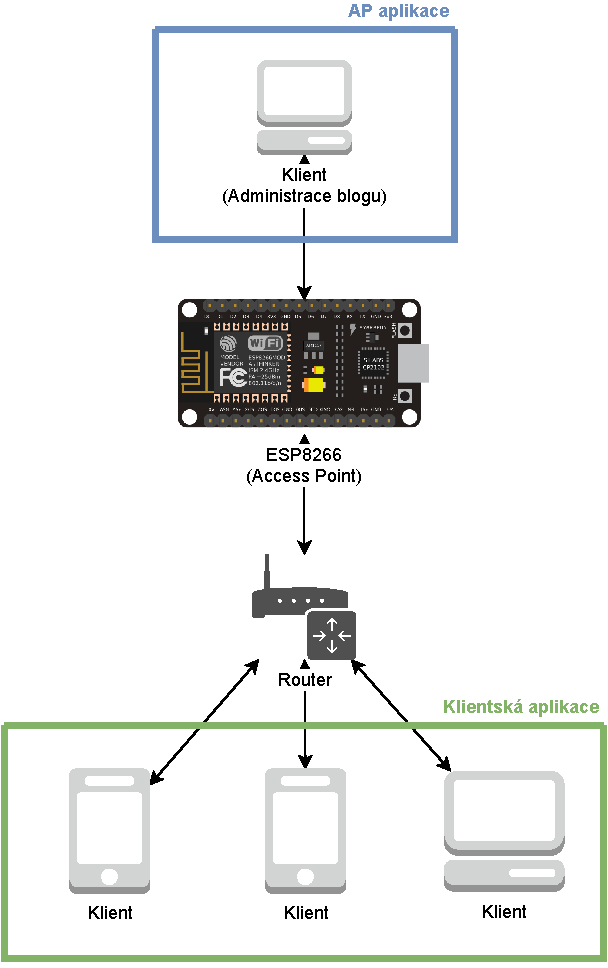
\includegraphics{images/app_communication_diagram.pdf}
	\caption{Komunikace mezi zařízeními}
\end{figure}

\subsection{AP Aplikace}
AP aplikace slouží pro administraci blogu. Je dostupná při připojení na Access Point na adrese \url{http://1.2.3.4} nebo na doméně, jejíž nastavení je popsáno dále (při prvním spuštění se jedná o adresu \url{http://blog/}). Pomocí doménového jména je možné se k aplikaci připojit díky DNS serveru, který běží také na ESP8266.

\begin{figure}[H]
	\centering
	\fbox{\includegraphics[scale=1]{images/admin_index.png}}
	\caption{Hlavní stránka (Access Point)}
\end{figure}

Aplikace umožňuje zobrazovat, mazat, vytvářet a upravovat články pomocí markdown editoru.

\begin{figure}[H]
	\centering
	\fbox{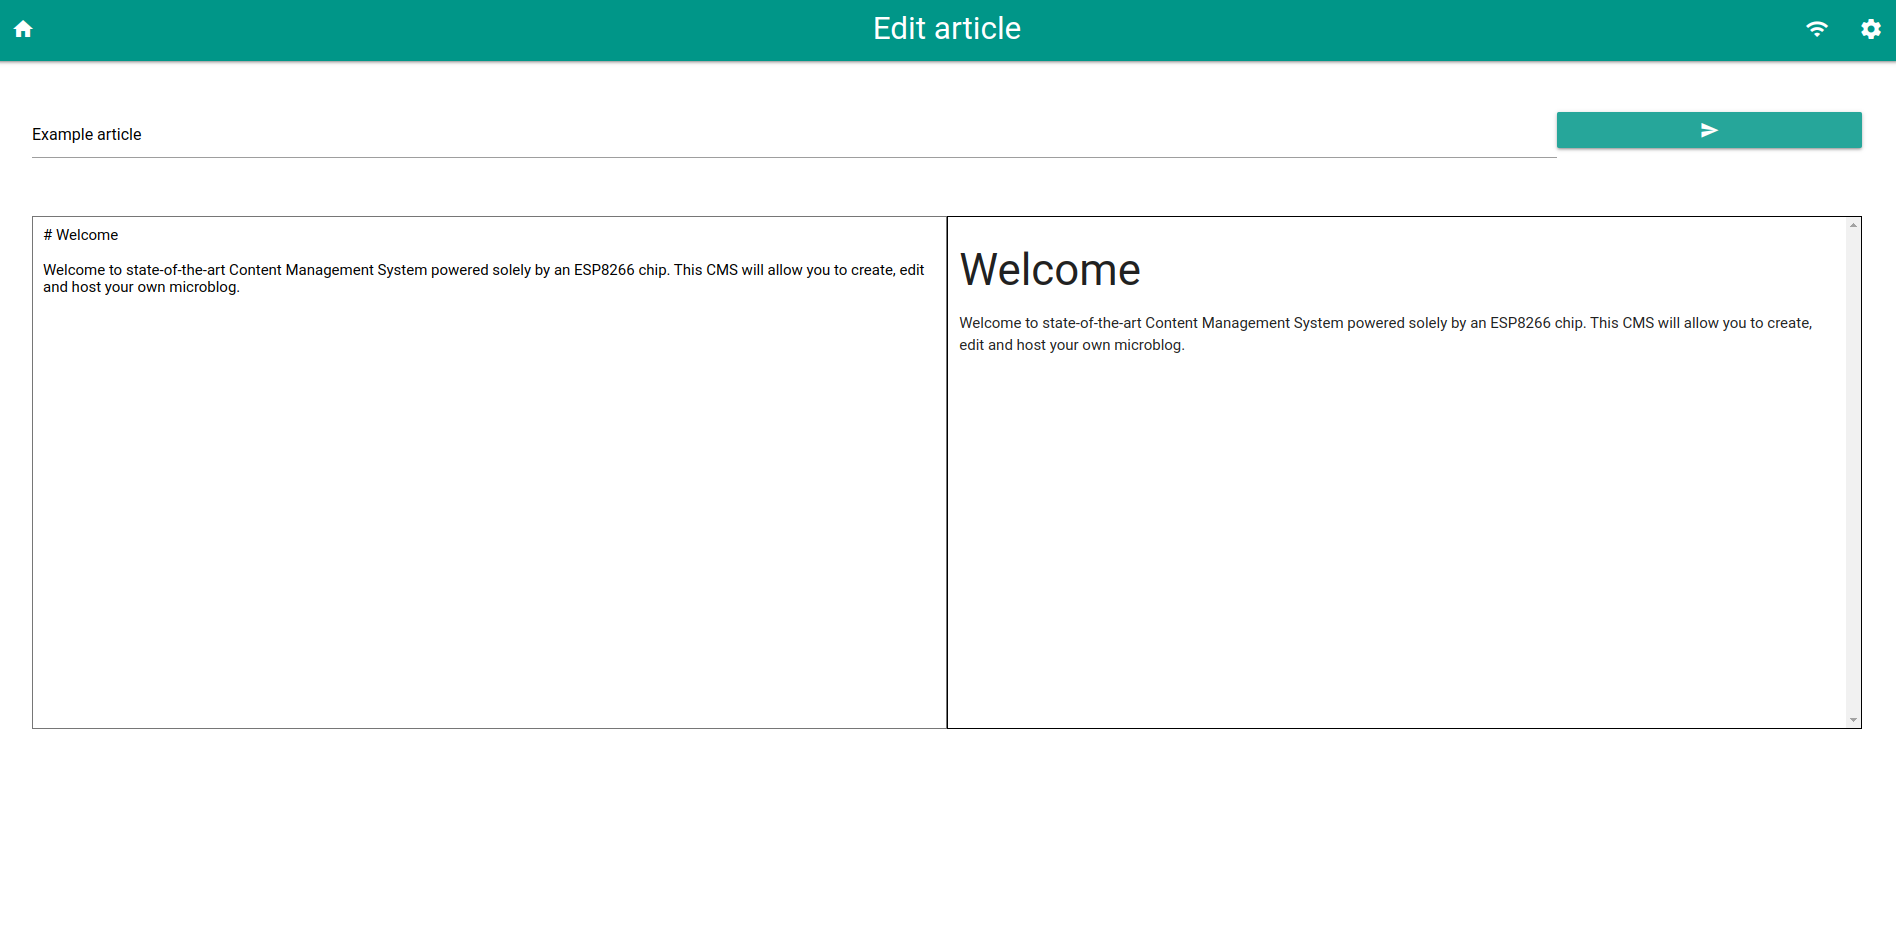
\includegraphics[scale=.25]{images/editor.png}}
	\caption{Editor (Access Point)}
\end{figure}

Její důležitou částí je i komponenta starající se o připojení k síti. Tato komponenta (v kódu se jedná o třídu \texttt{WifiManager}) spravuje jednotlivá připojení a ukládá údaje o známých sítích (ssid a heslo) do flash paměti, takže jsou dostupné i po restartu zařízení. Po restartu zařízení ho automaticky připojí na nějakou z uložených sítí, pokud je dostupná.

\begin{figure}[H]
	\centering
	\fbox{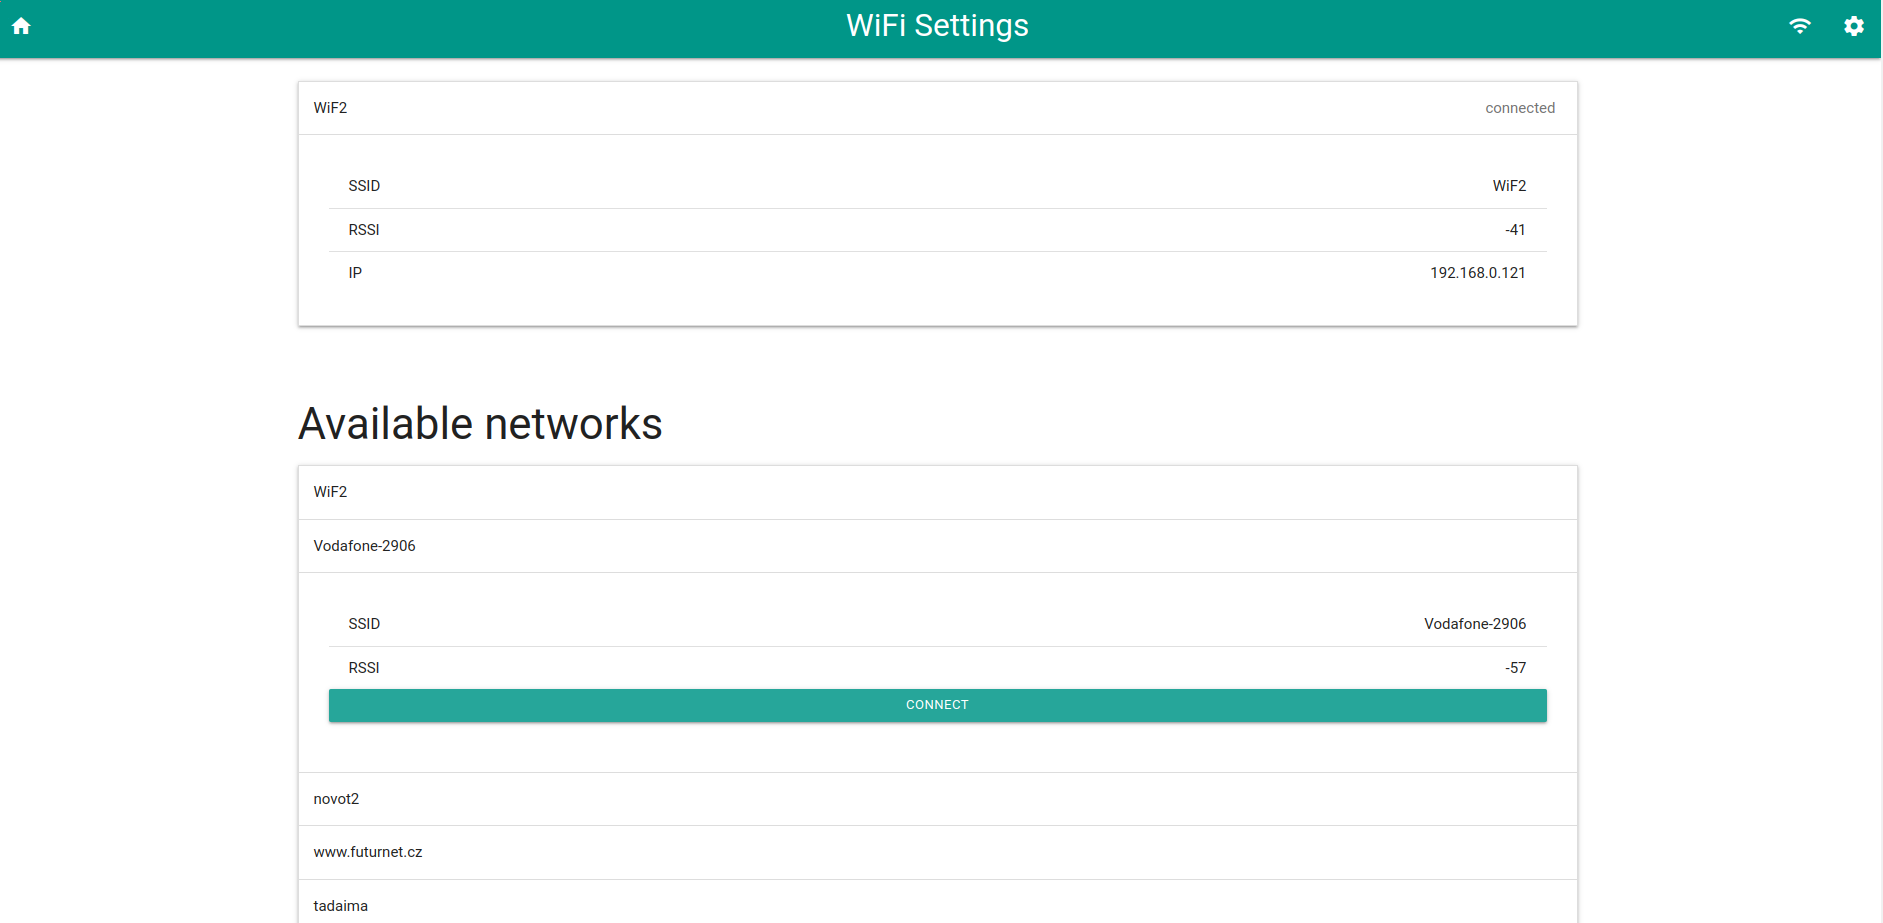
\includegraphics[scale=.25]{images/wifi_settings.png}}
	\caption{WiFi nastavení (Access Point)}
\end{figure}


Další důležitou částí AP Aplikace je obrazovka s nastavením, která umožňuje uživateli změnit jméno a heslo Access Pointu a doménové jméno, na kterém je aplikace dostupná.

\begin{figure}[H]
	\centering
	\fbox{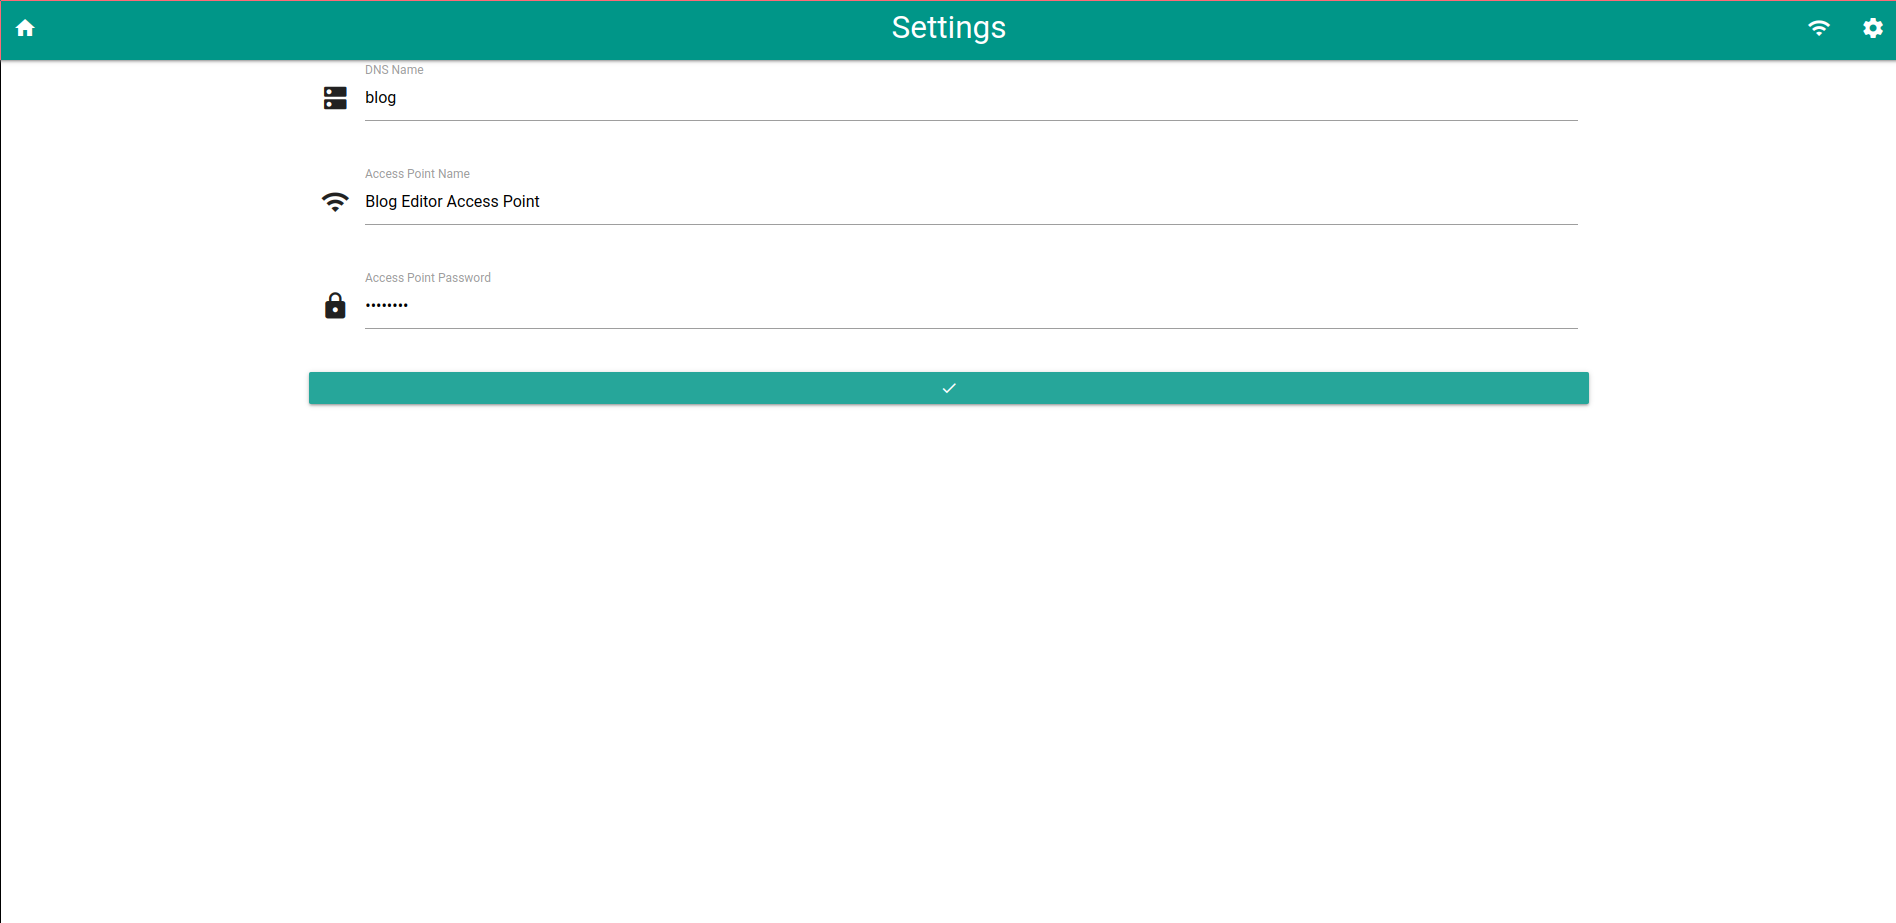
\includegraphics[scale=.25]{images/settings.png}}
	\caption{Nastavení (Access Point)}
\end{figure}

\subsection{Klientská aplikace}
Klientská aplikace, je uživateli prezentována při připojení mimo Access Point. Poskytuje rozhraní pro čtení vytvořených článků.

\begin{figure}[H]
	\centering
	\fbox{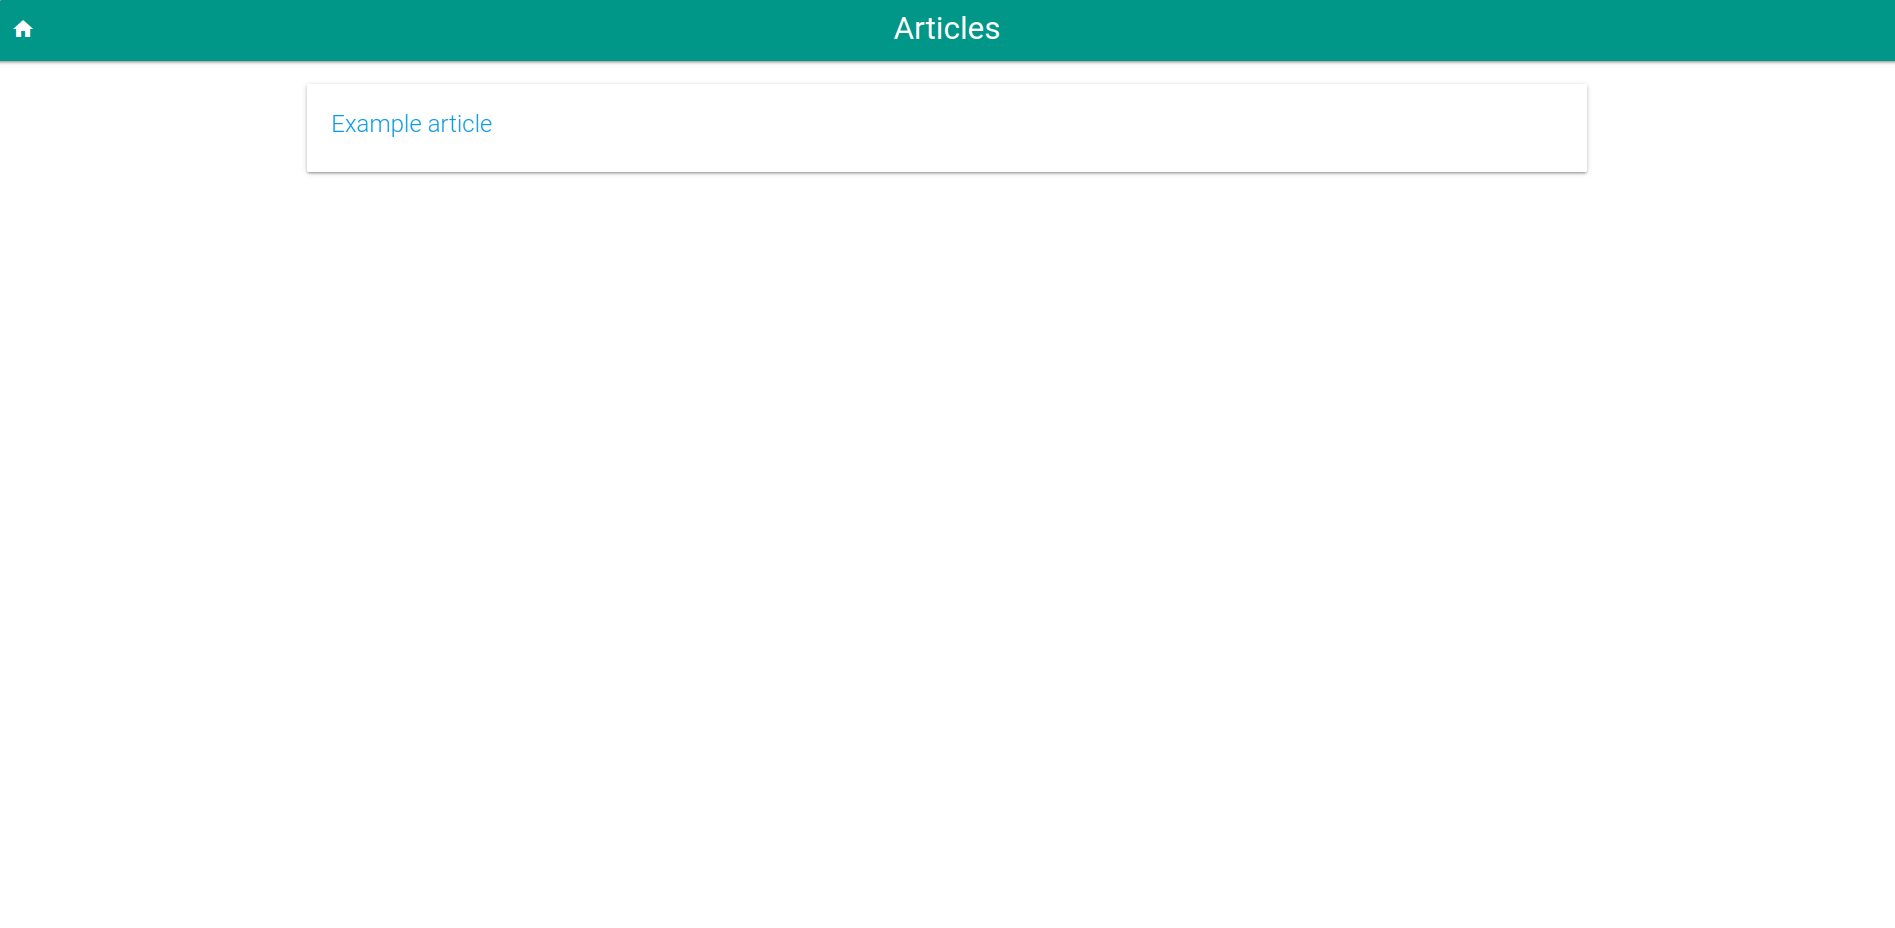
\includegraphics[scale=.25]{images/index.png}}
	\caption{Hlavní stránka (Klientská aplikace)}
\end{figure}

\begin{figure}[H]
	\centering
	\fbox{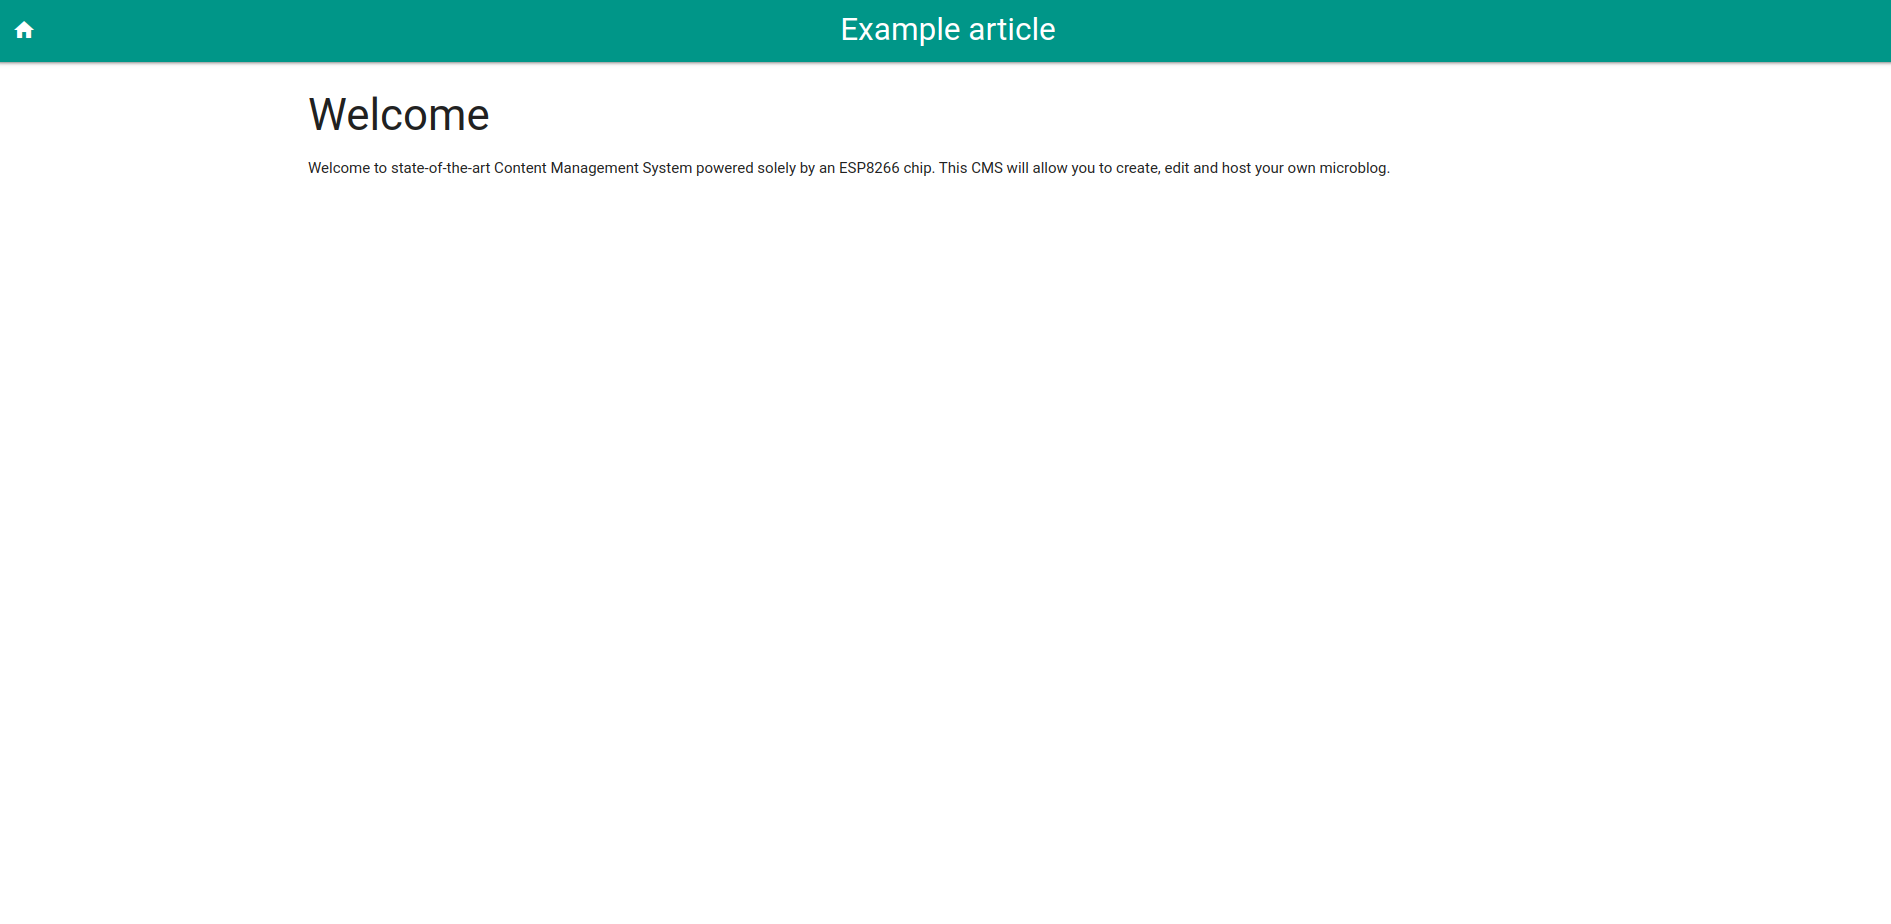
\includegraphics[scale=.25]{images/article.png}}
	\caption{Článek (Klientská aplikace)}
\end{figure}

\section{Závěr}
V rámci práce vznikl Content Management System, který je možné spustit na ESP8266. CMS umožňuje vytvářet, upravovat a sdílet články. Veškerý obsah hostovaného blogu a nastavení CMS je díky webovému rozhraní možné spravovat a konzumovat z jakéhokoli zařízení s webovým prohlížečem.

\end{document}
